In this chapter it will be illustrated a technique of control called \textbf{Nonlinear Model Predictive Control}. Other techniques we treated did not need some specific math tools in order to be explained and understood. This time we need some instruments that guide us to the study of this powerful and general control method.

\section{Math tools}
\subsection{Vector and signal norms}

{\color{blue} \subsubsection{Vector spaces}
}
\subsubsection{Vector spaces}
A \textbf{linear vector space } $F$ over a field $\mathbb{A}$ is a \textit{set} equipped of two operations: 
\begin{enumerate}
    \item \textbf{Vector addition}: $\forall f, g \ \in F \Leftarrow f+g\in F$
    \item \textbf{Scalar multiplication}: $\forall \alpha\in \mathbb{R}, \ f \in F \Leftarrow \alpha f \in F$
\end{enumerate}
Let us put together these two properties obtaining: 
{
\large{
    \begin{equation*}
    \forall \alpha, \beta \in \mathbb{R}, \ \forall f, g \in F \leftarrow 
    \alpha f + \beta g \in F
\end{equation*}
}
}
{\color{blue} \subsubsection{Norm: general definition} }

A \textbf{norm} is a function $\lVert  \diamond \rVert : \mathbb{R}^n\rightarrow\mathbb{R}$ which satisfies the following properties: 
\begin{enumerate}
    \item $\lVert x \rVert \ge 0$
    \item $ \Vert \alpha x \rVert = \alpha \lVert x \rVert$
    \item $\lVert x+y \rVert \le \lVert x \rVert + \lVert y \rVert $ (triangular inequality)
    \item $\lVert x \rVert=0 \Longleftrightarrow x=0$
\end{enumerate}
{\color{blue} \subsubsection{Vector norm}}

Let us consider a vector $f=(f_1, ..., f_n)^T\in\mathbb{R}^n$, we can define some norm functions in particular $\ell_1, \ell_2$ and $\ell_\infty$ norms:
\begin{itemize}
    \item \underline{$\ell_1$-norm} is defined as: $\lVert f \rVert_1=\sum_{i=1}^{n}\lvert f_i \rvert$ 
    \item \underline{$\ell_2$-norm} is defined as: 
    $\lVert f \rVert_2=\sqrt{\sum_{i=1}^n f_i^2}$
    \item \underline{$\ell_\infty$-norm} is defined as:
   $ \lVert f \rVert_\infty=\max_{i=1,..., n} \lvert f_i \rvert$
    \item \underline{$\ell_2$ weighted norm} is defined as: 
    $\lVert f \rVert_{Q,2}=\sqrt{f^T Q f}=\sqrt{\sum_{i=1}^n qi f_i^2}$
\end{itemize}
The last type of norm is used when one want to give more or less importance to a certain component in the vector.

{\color{red}In \textsc{Matlab}} the command in order to compute a norm of a vector $f$ properly defined is \texttt{norm(f)}, by default it is the $\ell_2$-norm if not specified, otherwise one should use the commands \texttt{norm(f,1)} to indicate the $\ell_1$-norm and \texttt{norm(f,inf)} in order to indicate the $\ell_\infty$-norm. \\
{\color{blue} \subsubsection{Signal norm}}

Another important type of norm is that of a \textbf{signal} which is defined in a similar way with respect to the vector case. We consider both the cases of \textit{scalar function} and \textit{vector valued} functions. The main difference wrt the vectors is the fact that we have integrals instead of summations, a function can be seen as a vector composed by an \textbf{infinite number of elements}. \\

\noindent
\textbf{First case: $f: \mathbb{R}\to \mathbb{R}$}.
We have the following definitions: 
\begin{align}
    &\Vert f(t) \Vert_1 = \int_{0}^{\infty} {\vert f(t) \vert \ dt} \quad (L_1-\text{norm})\\
    &\Vert f(t) \Vert_2 = \int_{0}^{\infty} {[f(t)]^2 \ dt} \quad (L_2-\text{norm})\\
    &\Vert f(t) \Vert_\infty =  \sup_{t\in\mathbb{R}^+} \vert f(t) \vert \quad (L_\infty-\text{norm}) \label{eq:f_inf}
\end{align}
{\color{red}In \textsc{Matlab}} it is a little bit more complicated to compute a norm of a function because at first we cannot treat infinite values with the computer. A way to overcome this fact is to define a variable \texttt{dt} as a \textit{sample step} and evaluate the function in a large number of points, then we can approximately calculate the norm by using the 'standard' command \texttt{norm}.
Then, we have for example: 
{\color{blue}
\begin{verbatim}
    dt=0.0001;
    t=linspace(0,100, dt); 
    f=sin(t); 

    L2   = norm(f,2)*sqrt(dt);       %L_2 norm
    L1   = norm(f,1)*dt;             %L_1 norm
    Linf = norm(f,inf);              %L_inf norm          
\end{verbatim}
}

The multiplicative terms \texttt{sqrt(dt)} and \texttt{dt} are been added in order to apply the definition. By doing the above calculations we have approximated the integrals.\\


\noindent
\textbf{Second case: $f:\mathbb{R}\to\mathbb{R}^n$}. This is the case of \textbf{vector-valued} functions in which $\forall t \in \mathbb{R}^+$ we have a vector $f(t)\in\mathbb{R}^n$. The definitions previously given are modified as follows (basically we have norms instead of absolute values due to the fact that for each $t$, you have a vector instead of a scalar): 
\begin{align}
    &\Vert f(t) \Vert_1 = \int_{0}^{\infty} \Vert f(t) \Vert_1 \ dt \quad (L_1-\text{norm})\\
    &\Vert f(t) \Vert_2 = \sqrt{\int_{0}^{\infty} \Vert f(t) \Vert_2^2 \ dt}=
    \sqrt{\int_{0}^{\infty} f(t)^Tf(t) \ dt } \quad (L_2-\text{norm})\\
    &\Vert f(t) \Vert_2 = \sup_{t\in\mathbb{R}^+} \Vert f(t) \Vert_\infty \quad (L_\infty-\text{norm}) \label{eq: fv_inf}\\ 
    &\Vert f(t) \Vert_{Q,2} = \sqrt{\int_{0}^{\infty} f(t)^T \ Q \ f(t) \ dt }  \quad (L_1 \  \text{weighted norm})
\end{align}
An observation can be done on (\ref{eq:f_inf}) and (\ref{eq: fv_inf}): the $\sup$ generalizes the concept of maximum, in particular a function might not assume the value of the maximum. \\
{\color{red}In \textsc{Matlab}} the \textbf{weighted $\ell_2$-norm} can be computed as follows:

{\color{blue}
\begin{verbatim}
    dt=0.0001; 
    t=linspace(0,100, dt);  
    f=[exp(-3*t); sin(3*t)];        %vector valued function 
    Q=diag(1,2,3); 
    
    L2 = sqrt( sum ( sum (Q*f.^2) * dt ) );
    %           ^     ^
    %           |     |
    %         \int   l2-norm
\end{verbatim}

}


\subsection{Optimization}
\textbf{Optimization} is a branch of Maths that deals with \textbf{finding the best solution to a problem} which is \textit{finding the minimum} of a function. Optimization acts a fundamental role in many engineering field and also in \textbf{control design} is important: when we design a controller we want to: (i) minimize the tracking error; (ii) minimize the command effort as the actuators has got limited working ranges; (iii) minimize the effect of disturbances. In our case we introduce it, in order to apply it to \textit{Model Predictive Control}.

{\color{blue}\subsubsection{Basic notions}}
In the \textbf{univariate function} $f: \mathbb{R}\to\mathbb{R}$ the problem of minimization is the following: 
{\large{

\begin{align}
   &x^*=\text{arg}\min_{x\in\mathbb{R}} f(x) \label{eq:minimizer}\\
    &f(x^*)=\min_{x\in\mathbb{R}} f(x) \label{eq: minimum}
\end{align}

}}

The (\ref{eq:minimizer}) is called the \textbf{minizer} while the (\ref{eq: minimum}) is called the \textbf{minimum}. The $x$ is the \textbf{decision variable}, while $f(\diamond)$ is called either the \textbf{objective function} or \textbf{cost function} or \textbf{loss function} (used in AI).\\
In a univariate problem there could be: \textit{one global minimum}, \textit{several global minima}, \textit{infinite global minima}. The optimization problems usually require that the solution (minimizer) observes some \textbf{constraints}, in this case we are talking about \textbf{constrained minimization}. As the constraints could be more than one, an alternative notation for the problem (\ref{eq:minimizer}) is:

{\large{
\begin{equation}
    \begin{aligned}
        \min \ &f(x)\\
        &\text{subject to} \ x\in \mathbb{R}
    \end{aligned}
\end{equation}

}}

Where \textit{subject to} is often abbreviated as \textbf{s.t.}\\
In order to start talking about optimization we considered the \textbf{univariate} case in which the decision is taken according a \textbf{single variable}, in engineering problems the decision variable can be hundreds or thousands! The graphical representation becomes not possible at all, but the concepts we exposed previously remain more or less the same but more general. We are talking about in this case of \textbf{multivariate functions}. In particular: 
\begin{itemize}
    \item The \textbf{objective function} $f(x)$ is such that $f:\mathbb{R}^n\to\mathbb{R}$
    \item The \textbf{decision variable} is a vector $x\in\mathbb{R}^n$
    \item Also the \textbf{minimizer} is a vector $x^*\in \mathbb{R}^n$
\end{itemize}
An Optimization problem is said to be \textbf{feasible} if there is at least a solution, otherwise it is said to be \textbf{unfeasible}. We can define in this way a \textbf{feasible set} as:
{\large{

\begin{equation}
    \mathcal{X}^*=\{x^* \in \mathbb{R}^n \ : p=f(x^*) \}
\end{equation}
}}

where $p$ is the minimum. We can immediately understand that when an optimization problem is \textit{unfeasible} is such that $\mathcal{X}^*=\emptyset$. \\
Surely a nice class of optimization problems is the \textbf{convex optimization} class.

{\color{blue} \subsubsection{Minimization}}

\section{Introduction to NMPC}
\textbf{Nonlinear Model Predictive Control (NMPC)} is a general control methods which differently than the others that has been treated, provide us with a way for taking into account both the aspects related to: 
\begin{itemize}
    \item \textbf{Constraints} which are applied either on input, state or output; 
    \item \textbf{Trade off between performance and command activity} which is managed in a systematic way how will be seen.
\end{itemize}
The \textbf{Approach} of this control technique is the following. At each time step: 
\begin{enumerate}
    \item A prediction \textbf{over a given time horizon} is performed using a model of the plant; 
    \item The command input is chosen as the one yielding the "best" prediction, that is the closer to the specified behaviour and this is done by solving an \textbf{online optimization algorithm}
\end{enumerate}

This time the mathematical form of the plant is not assumed to be \textbf{affine} like in the Feedback linearization and Sliding Mode control, but it is in general a MIMO system characterized by
\begin{equation} \label{eq: MIMO_system}
    \begin{aligned}
        &\dot{x}=f(x,u)\\
        &y=h(x,u)
    \end{aligned}
\end{equation}
where $x, y$ and $u$ are as usual the state, the output and the input. A generalization to time varying systems could be done without particular efforts.\\
The state is measured in \textbf{real time}, with a proper sampling time $T_s$. The measurement are:
$$x(t_k), \ t_k=T_sk, \  k=0,1, ...$$
If the state cannot be measured an observer has to be employed. 

\section{First step: Prediction}
At each time $t=t_k$ both the \textbf{state} $\hat{x}(\tau)$ and the \textbf{output} $\hat{y}(\tau)$ are predicted over the time interval $[t, t+T_p]$ by integrating (\ref{eq: MIMO_system}). The time $T_p \ge T_s$ is called the \textbf{prediction horizon}. For each $\tau\in [t,t+T_p]$, the quantity $\hat{y}(\tau)$ (the \textbf{predicted output}) depends on:
\begin{itemize}
    \item The \textbf{initial state} $x(t)$
    \item The \textbf{input signal} $u(t:\tau)$ which denotes a generic input signal in the interval $[t, \tau]$, this is an \textbf{open-loop} signal in the sense that it depends on the initial state $x(t)$, but not on $x(\tau)$ that is the "current" state.
\end{itemize}

\section{Second step: Optimization}
At each time $t=t_k$ we find an \textbf{input signal} $u(t:\tau)=u^*(t:\tau)$ such that the \underline{prediction}  
$$
    \hat{y}(x(t), u^*(t:\tau))\equiv \hat{y}(u^*(t:\tau))
$$
has the \underline{desired behaviour} for all $\tau \in [t, t+T_p]$. We seek a signal that for each sub-interval $[t,\tau]$ gave the desired behaviour. This concept is formalize by defining the objective function   \\

\hspace*{-5mm}
\begin{tikzpicture}
\node [mybox] (box){%
    \begin{minipage}{.96\textwidth}     %Larghezza del box
        {\large{
        \begin{equation*}
            J(u(t:t+T_p)) = \int_{t}^{t+T_p} {(\Vert \Tilde{y}(\tau) \Vert_Q^2 + \Vert u(\tau) \Vert_R^2 )  \ d\tau} + \Vert \Tilde{y}(t + T_p) \Vert_P
        \end{equation*}
        
        }}
    \end{minipage}
};
\end{tikzpicture}%


the term $\tilde{y}(\tau)=r(\tau)-\hat{y}(\tau)$ is the \textbf{predicted tracking error}, $r(\tau)\in\mathbb{R}^{n_y}$ is a \textbf{reference to track}, while $\Vert \diamond \Vert_X$ is the \textbf{weighted norm}. The input $u^*(t:t+T_p)$ is chosen as one \textbf{minimizing} the objective function $J(u(t:t+T_p))$, in which:
\begin{itemize}
    \item The term $\Vert \tilde{y}(\tau) \Vert_Q^2$ is for minimizing the tracking error over a finite interval; 
    \item The term $\Vert \tilde{y}(t+T_p) \Vert_P^2$ gives importance to the final tracking error; 
    \item Finally the term $\Vert u(\tau) \Vert_R^2$ allows us to manage in a systematic way the performance beetween command activity and performances. 
\end{itemize}

The predicted tracking error $\tilde{y}(\tau)$ depends on the \textit{predicted output} which is derived from the integration of (\ref{eq: MIMO_system}), so the \textbf{minimization of the functional $J$} is therefore subject to the constraints:
\begin{align*}
    &\dot{\hat{x}}(\tau)=f(\hat{x}(\tau), u(\tau)), \ \hat{x}(t)=x(t), \tau\in[t, t+T_p]\\
    &\hat{y}(\tau)=h(\hat{x}(\tau), u(\tau)) 
\end{align*}
Other constraints can be present on:
\begin{itemize}
    \item The output or the state (eg. collision avoidance, obstacles) so that we have $\hat{x}(\tau) \in X_c$ and $\hat{y}(\tau)\in Y_c$; 
    \item The input (eg. input saturation) so that we have $u(\tau) \in U_c$;
\end{itemize}
The image below \textbf{summarizes} the steps of NMPC which are done for each $t=t_k$ many feasible solutions {\color{blue} $u(t:t+Tp)$} are provided, in the \textbf{prediction step}, relative predicted output and state are computed by using a model of the plant, for each of these choices I compute the quantity $J(u(t:t+T_p)$, finally in the \textbf{optimization step}, I select the best choice {\color{red} $u^*(t:t+T_p)$}. 

\begin{figure}[h]
    \centering
    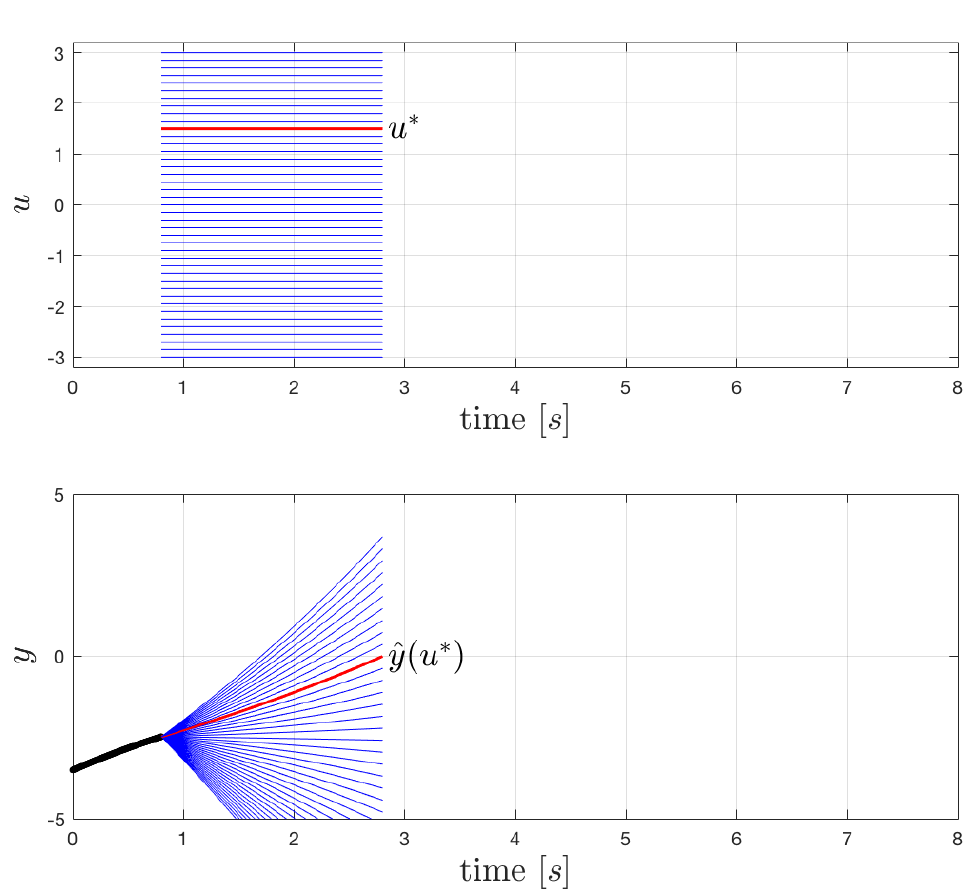
\includegraphics[scale=0.6]{NonLinearControl/images/NMPC_graph.png}
    \caption{Example of a step of Prediction and Minimization}
    \label{fig:enter-label}
\end{figure}

For each $t=t_k$ and $\tau \in [t, t+T_p]$ the following \textit{optimization problem} is solved:\\

\hspace*{-5mm}
\begin{tikzpicture}
\node [mybox] (box){%
    \begin{minipage}{.96\textwidth}     %Larghezza del box
    {\large{
\begin{equation} \label{eq:opt_alg}
    \begin{aligned}
        &u^*(t:t+T_p)=\text{arg}\min_{u(\cdot)} J(u(t:t+T_p)\\
        &\text{subject to:}\\
        &\dot{\hat{x}}(\tau)=f(\hat{x}(\tau), u(\tau)), \ \hat{x}(t)=x(t)  \quad (\text{\small{initial conditions)}}\\
        &\hat{y}(\tau)=h(\hat{x}(\tau), u(\tau)) \\
        &\hat{x}(\tau) \in \mathcal{X}_c, \ \hat{y}(\tau)\in \mathcal{Y}_c, \ u(\tau) \in \mathcal{U}_c
    \end{aligned}   
\end{equation}
}}
    \end{minipage}
};
\end{tikzpicture}%


where $T_s$  is the sampling time, $T_p\ge T_s$ is the \textbf{prediction horizon}. The exposed optimization problem is in general \textbf{non-convex} moreover must be solved online. Usually such optimization problem is solved by using efficient numerical algorithms. 

\section{Reciding Horizon}
Suppose that at a certain time $t=t_k$, the problem (\ref{eq:opt_alg}) is solved and a $u^*
(t:t+T_p)$ is found, as we mentioned this is an open-loop input,in fact it depends on $x(t)$, but not on $x(\tau), \tau>t$. For this reason If we applied this input in the whole interval $[t, t+T_p]$, we would not have be able to \textbf{increase the precision} or \textbf{adapt to a varying scenario}. At this point the \textbf{NMPC feedback control algorithm} is obtained applying the so-called \textit{receding horizon strategy}:\\

\hspace*{-5mm}
\begin{tikzpicture}
\node [mybox] (box){%
    \begin{minipage}{.96\textwidth}     %Larghezza del box
        \begin{enumerate}
            \item At each time $t=t_k$
            \begin{itemize}
                \item The problem (\ref{eq:opt_alg}) is solved
                \item Apply only the first input value $u(\tau)=u^*(t=t_k)$ and keep it constant for each $\tau \in [t_k, t_{k+1}]$
            \end{itemize}
            \item Repeat the preceding steps for  $t=t_{k+1}, t_{k+2},...$
        \end{enumerate}
    \end{minipage}
};
\end{tikzpicture}%


 
\section{Closed-loop scheme}
As it has been done in the explanation of the previous techniques of Nonlinear control, now we show the control scheme for a plant controlled by using the NMPC technique. 
The \textbf{plant} is in the form (\ref{eq: MIMO_system}), the block \textbf{NMPC} contains an on-line algorithm which solve the optimization problem and apply the \textit{reciding horizon strategy}.

\begin{figure}[h]
    \centering
    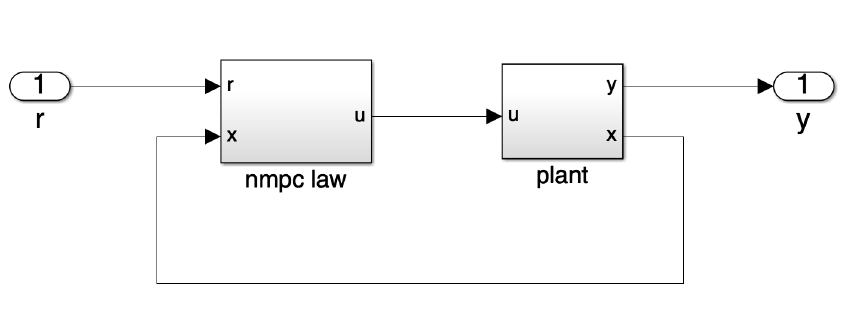
\includegraphics{NonLinearControl/images/NMPC_CtrlScheme.png}
    \caption{Control Scheme for NMPC}
    \label{fig:enter-label}
\end{figure}

\section{NMPC design}

\subsection{Choice of the parameters}
\begin{itemize}
    \item $\mathbf{T_s}$, sufficiently small in order to respect the Nyquist-Shannon Theorem, but not too small this would result in slow computation; sometimes cannot be chosen.
    \item $\mathbf{T_p}$ it is determined through a trial and error procedure in simulation keeping in mind that a "large" $T_p$ increases the \textbf{closed-loop stability}, a "too large" $T_p$ would result in reducing in the \textbf{short-time tracking accuracy}.
\end{itemize}

\subsection{Choice of the weight matrices}
The \textbf{initial choice} of the \textbf{weight matrices} $Q, R, P$ can be diagonal non negative  such that \\

\hspace*{-5mm}
\begin{tikzpicture}
\node [mybox] (box){%
    \begin{minipage}{.96\textwidth}     %Larghezza del box
        \begin{align*}
    &Q_{ii}=\begin{cases}
        >0 & \text{in the presence of requirements  on} y_i\\
        =0  & \text{otherwise}
    \end{cases}\\
     &R_{ii}=\begin{cases}
        >0 & \text{in the presence of requirements  on} u_i\\
        =0  & \text{otherwise}
    \end{cases}\\
     &P_{ii}=\begin{cases}
        >0 & \text{in the presence of requirements  on} y_i\\
        =0  & \text{otherwise}
    \end{cases}
\end{align*}
    \end{minipage}
};
\end{tikzpicture}%


The weight matrices can be tuned by \textbf{trial/error procedure} considering that: 
\begin{itemize}
    \item Increasing $Q_{ii}, P_{ii} \Rightarrow$ decreasing of the energy of $x_i, y_i \Rightarrow$ reducing \textbf{oscillations} and \textbf{convergence time}; 
    \item Increasing $R_{ii} \Leftarrow$ decreasing of the energy of $u_i \Leftarrow$ reducing \textbf{command effort} and \textbf{energy consumption}. 
\end{itemize}

\section{Discussion: pros and cons}